%\input{Preambulum}

\begin{figure}[t!]
\centering
\begin{subfigure}{0.3\textwidth}
\centering
\caption{$G_1$: $1$ excl., \#6}
\label{Fig3a}

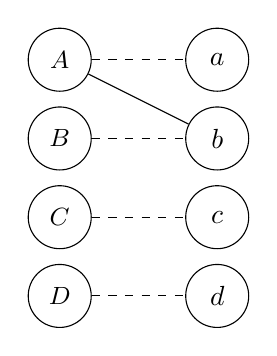
\begin{tikzpicture}[scale=1, auto=center]
\tikzstyle{every node}=[draw,shape=circle];
  \node[minimum size=0.8cm] (n1) at (0,3) {\small{$A$}};
  \node[minimum size=0.8cm] (n2) at (0,2) {\small{$B$}};
  \node[minimum size=0.8cm] (n3) at (0,1) {\small{$C$}};
  \node[minimum size=0.8cm] (n4) at (0,0) {\small{$D$}};
  \node[minimum size=0.8cm] (n5) at (2,3) {$a$};
  \node[minimum size=0.8cm] (n6) at (2,2) {$b$};
  \node[minimum size=0.8cm] (n7) at (2,1) {$c$};
  \node[minimum size=0.8cm] (n8) at (2,0) {$d$};

  \foreach \from/\to in {n1/n5,n2/n6,n3/n7,n4/n8}
    \draw[dashed] (\from) -- (\to);
  \foreach \from/\to in {n1/n6}
    \draw (\from) -- (\to);
\end{tikzpicture}
\end{subfigure}
\begin{subfigure}{0.3\textwidth}
\centering
\caption{$G_2$: $2$ excl., \#4}
\label{Fig3b}

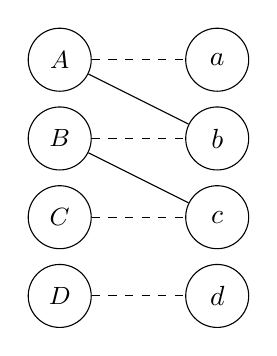
\begin{tikzpicture}[scale=1, auto=center]
\tikzstyle{every node}=[draw,shape=circle];
  \node[minimum size=0.8cm] (n1) at (0,3) {\small{$A$}};
  \node[minimum size=0.8cm] (n2) at (0,2) {\small{$B$}};
  \node[minimum size=0.8cm] (n3) at (0,1) {\small{$C$}};
  \node[minimum size=0.8cm] (n4) at (0,0) {\small{$D$}};
  \node[minimum size=0.8cm] (n5) at (2,3) {$a$};
  \node[minimum size=0.8cm] (n6) at (2,2) {$b$};
  \node[minimum size=0.8cm] (n7) at (2,1) {$c$};
  \node[minimum size=0.8cm] (n8) at (2,0) {$d$};

  \foreach \from/\to in {n1/n5,n2/n6,n3/n7,n4/n8}
    \draw[dashed] (\from) -- (\to);
  \foreach \from/\to in {n1/n6,n2/n7}
    \draw (\from) -- (\to);
\end{tikzpicture}
\end{subfigure}
\begin{subfigure}{0.3\textwidth}
\centering
\caption{$G_3$: $2$ excl., \#3}
\label{Fig3c}

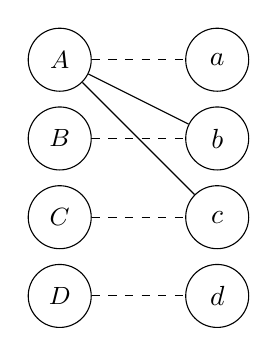
\begin{tikzpicture}[scale=1, auto=center]
\tikzstyle{every node}=[draw,shape=circle];
  \node[minimum size=0.8cm] (n1) at (0,3) {\small{$A$}};
  \node[minimum size=0.8cm] (n2) at (0,2) {\small{$B$}};
  \node[minimum size=0.8cm] (n3) at (0,1) {\small{$C$}};
  \node[minimum size=0.8cm] (n4) at (0,0) {\small{$D$}};
  \node[minimum size=0.8cm] (n5) at (2,3) {$a$};
  \node[minimum size=0.8cm] (n6) at (2,2) {$b$};
  \node[minimum size=0.8cm] (n7) at (2,1) {$c$};
  \node[minimum size=0.8cm] (n8) at (2,0) {$d$};

  \foreach \from/\to in {n1/n5,n2/n6,n3/n7,n4/n8}
    \draw[dashed] (\from) -- (\to);
  \foreach \from/\to in {n1/n6,n1/n7}
    \draw (\from) -- (\to);
\end{tikzpicture}
\end{subfigure}

\vspace{0.25cm}
\begin{subfigure}{0.3\textwidth}
\centering
\caption{$G_4$: $3$ excl., \#3}
\label{Fig3d}

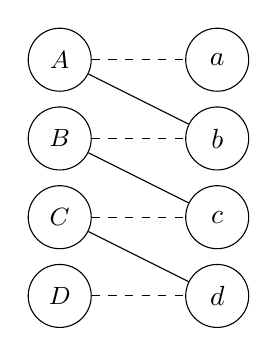
\begin{tikzpicture}[scale=1, auto=center]
\tikzstyle{every node}=[draw,shape=circle];
  \node[minimum size=0.8cm] (n1) at (0,3) {\small{$A$}};
  \node[minimum size=0.8cm] (n2) at (0,2) {\small{$B$}};
  \node[minimum size=0.8cm] (n3) at (0,1) {\small{$C$}};
  \node[minimum size=0.8cm] (n4) at (0,0) {\small{$D$}};
  \node[minimum size=0.8cm] (n5) at (2,3) {$a$};
  \node[minimum size=0.8cm] (n6) at (2,2) {$b$};
  \node[minimum size=0.8cm] (n7) at (2,1) {$c$};
  \node[minimum size=0.8cm] (n8) at (2,0) {$d$};

  \foreach \from/\to in {n1/n5,n2/n6,n3/n7,n4/n8}
    \draw[dashed] (\from) -- (\to);
  \foreach \from/\to in {n1/n6,n2/n7,n3/n8}
    \draw (\from) -- (\to);
\end{tikzpicture}
\end{subfigure}
\begin{subfigure}{0.3\textwidth}
\centering
\caption{$G_5$: $3$ excl., \#3}
\label{Fig3e}

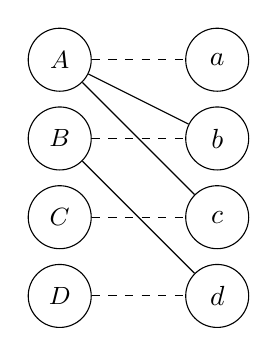
\begin{tikzpicture}[scale=1, auto=center]
\tikzstyle{every node}=[draw,shape=circle];
  \node[minimum size=0.8cm] (n1) at (0,3) {\small{$A$}};
  \node[minimum size=0.8cm] (n2) at (0,2) {\small{$B$}};
  \node[minimum size=0.8cm] (n3) at (0,1) {\small{$C$}};
  \node[minimum size=0.8cm] (n4) at (0,0) {\small{$D$}};
  \node[minimum size=0.8cm] (n5) at (2,3) {$a$};
  \node[minimum size=0.8cm] (n6) at (2,2) {$b$};
  \node[minimum size=0.8cm] (n7) at (2,1) {$c$};
  \node[minimum size=0.8cm] (n8) at (2,0) {$d$};
  
  \foreach \from/\to in {n1/n5,n2/n6,n3/n7,n4/n8}
    \draw[dashed] (\from) -- (\to);
  \foreach \from/\to in {n1/n6,n1/n7,n2/n8}
    \draw (\from) -- (\to);
\end{tikzpicture}
\end{subfigure}
\begin{subfigure}{0.3\textwidth}
\centering
\caption{$G_6$: $4$ excl., \#3}
\label{Fig3f}

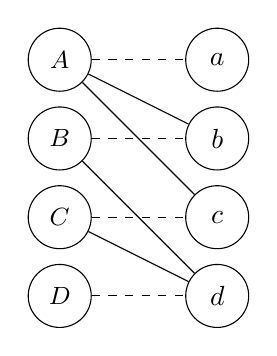
\begin{tikzpicture}[scale=1, auto=center]
\tikzstyle{every node}=[draw,shape=circle];
  \node[minimum size=0.8cm] (n1) at (0,3) {\small{$A$}};
  \node[minimum size=0.8cm] (n2) at (0,2) {\small{$B$}};
  \node[minimum size=0.8cm] (n3) at (0,1) {\small{$C$}};
  \node[minimum size=0.8cm] (n4) at (0,0) {\small{$D$}};
  \node[minimum size=0.8cm] (n5) at (2,3) {$a$};
  \node[minimum size=0.8cm] (n6) at (2,2) {$b$};
  \node[minimum size=0.8cm] (n7) at (2,1) {$c$};
  \node[minimum size=0.8cm] (n8) at (2,0) {$d$};

  \foreach \from/\to in {n1/n5,n2/n6,n3/n7,n4/n8}
    \draw[dashed] (\from) -- (\to);
  \foreach \from/\to in {n1/n6,n1/n7,n2/n8,n3/n8}
    \draw (\from) -- (\to);
\end{tikzpicture}
\end{subfigure}

\caption{Balanced bipartite graphs with eight nodes where \\ the UEFA mechanism is unfair under the group constraints \\ \vspace{0.2cm}
\footnotesize{\emph{Notes}: Dashed lines indicate the group constraints, solid lines indicate the association constraints. \\
Group winners are the nodes on the left-hand side, runners-up are the nodes on the right-hand side. \\
excl. = (number of) exclusion(s); \# = number of valid assignments}}
\label{Fig3}
\end{figure}

%\end{document}